
\subsubsection{07.10.14}

\begin{enumerate}
	\item The time of beginning and ending of the meeting:
	17:00 - 21:30
	\item Purposes of the meeting:
	\begin{enumerate}
		\item Writе a program to control the robot by joystick.
		
		\item Begin creating the lift.
		
	\end{enumerate}
	\item Work, that has been done:
	\begin{enumerate}
		\item Control of the robot by joystick was implemented. Motor control is carried out by the left stick. During the tests we found that when a small current was supplied on motors, they could not be rotate and are too loud, leading us to conclude that they are only wearing out. Because of this it was decided to put a limit to how small the signal could be.
		
		\item  In order to raise the basket to 120 cm, it was decided to assemble two guides, each of which consists of four furniture rails: two by 30 cm and two by 35 cm. Thus the lifting height is 130 cm. The guides were installed on the robot.
		
		\begin{figure}[H]
			\begin{minipage}[h]{0.31\linewidth}
				\center{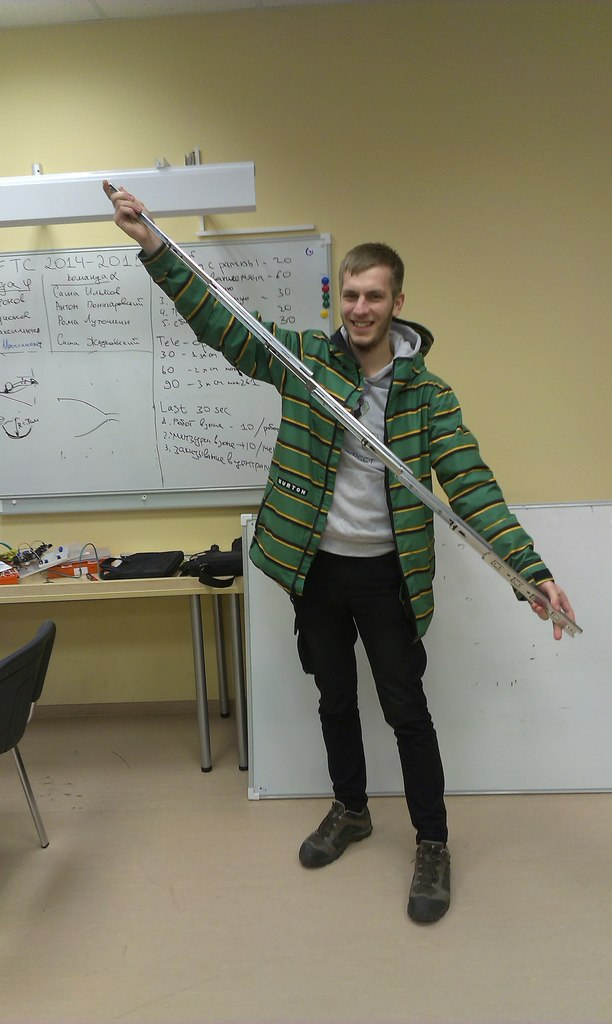
\includegraphics[scale=0.25]{days/07.10.14/images/01}}
			\end{minipage}
			\hfill
			\begin{minipage}[h]{0.31\linewidth}
				\center{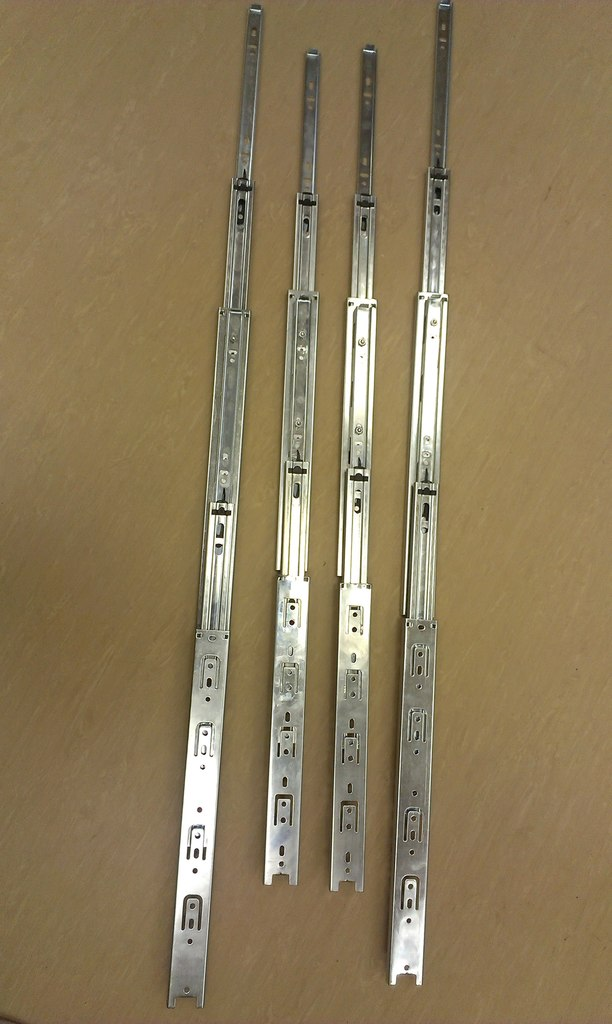
\includegraphics[scale=0.2]{days/07.10.14/images/02}}
			\end{minipage}
			\hfill
			\begin{minipage}[h]{0.31\linewidth}
				\center{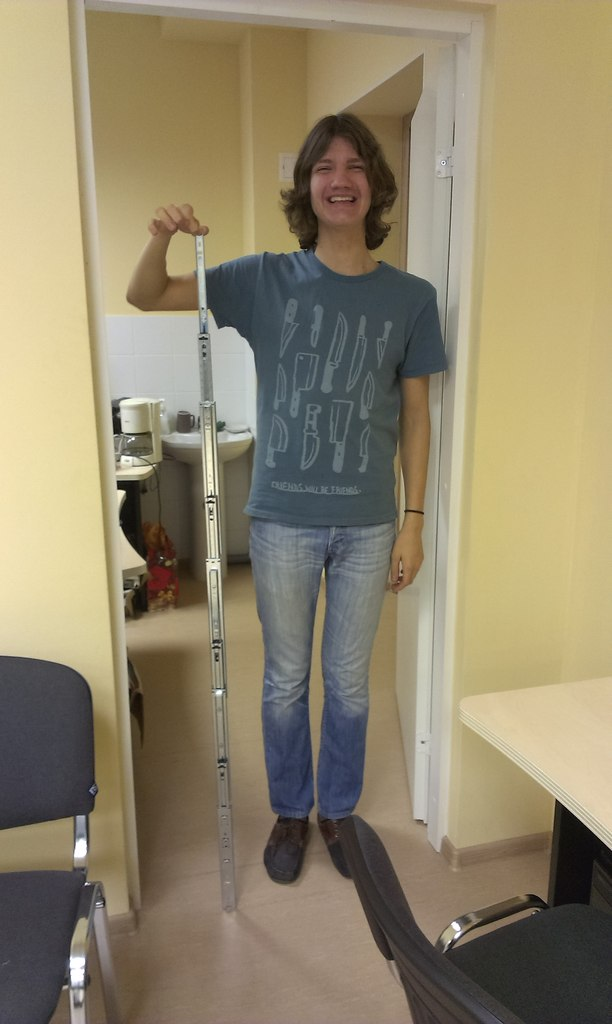
\includegraphics[scale=0.25]{days/07.10.14/images/03}}
			\end{minipage}
			\caption{Guides for the lift}
		\end{figure}
		
		\item It was decided to install a lift in the central part of the robot. Electronics were installed in the rear part and protected from damage by the lifting mechanism. Some space was left for the bucket in the front of the robot. 
		
		\item Since the bucket is lowered inside the robot, it is protected from collisions. But in this case, the location of the bucket raises the question of how the balls will get into the bucket. It was decided to increase the distance between the floor and the bottom of the front frame of beam to 7 cm so that a big ball could go. This was achieved by turning the motors around in their mounts. In addition, this decision to increase clearance increased the stability of the robot.
		
		\begin{figure}[H]
			\begin{minipage}[h]{1\linewidth}
				\center{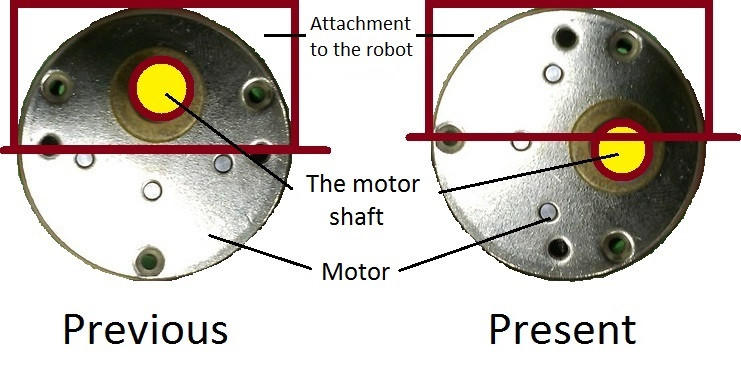
\includegraphics[scale=0.3]{days/07.10.14/images/04}}
				\caption{Increase clearance} 
			\end{minipage}
		\end{figure}
		
		\item In front of the robot we decided to install a soft brush, such as those installed on snow-clearing machines, that will rotate and capture balls. In the case when the robot has collected the maximum number of balls, the operator can stop the rotation of the brushes so other balls will not accidentally get into the bucket.
		
		\begin{figure}[H]
			\begin{minipage}[h]{0.47\linewidth}
				\center{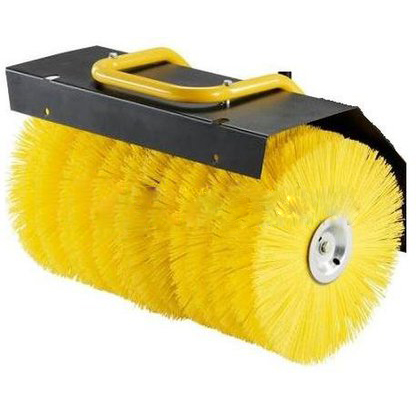
\includegraphics[scale=0.3]{days/07.10.14/images/05}}
			\end{minipage}
			\hfill
			\begin{minipage}[h]{0.47\linewidth}
				\center{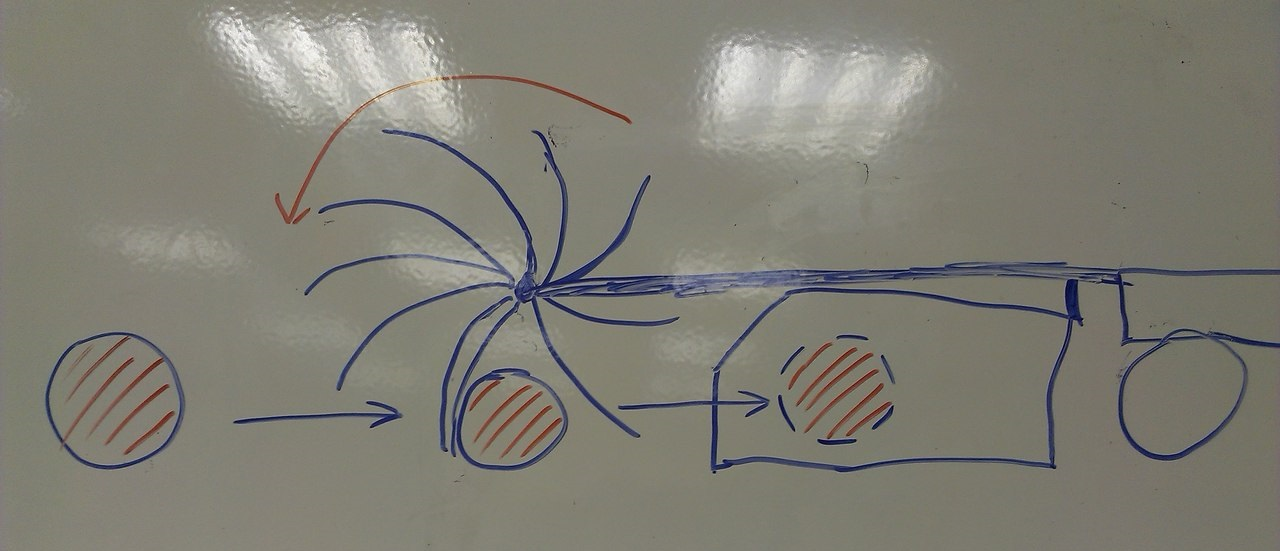
\includegraphics[scale=0.2]{days/07.10.14/images/06}}
			\end{minipage}
			\vfill
			\begin{minipage}[h]{0.47\linewidth}
				\center appearance
			\end{minipage}
			\hfill
			\begin{minipage}[h]{0.47\linewidth}
				\center The principle of operation
			\end{minipage}
			\caption{The idea to capture balls}
		\end{figure}
		
	\end{enumerate}
	
	\item Results:  
	\begin{enumerate}
		\item Implemented a simple program to control the robot.
		
		\item  Created and assigned rails for the lift.
		
		\item  Battery and motor drivers are properly fixed on the robot. NXT block has not been fixed, as it requires periodical removal for battery replacement.
		
		\item Clearance of the robot has been increased.
		
	\end{enumerate}
	
	\item Tasks for the next meetings:
	\begin{enumerate}
		\item To finish the program of robot control.
		
		\item To implement control of the robot by Bluetooth.
		
		\item To create a mechanism for moving the guides apart.
		
	\end{enumerate}     
\end{enumerate}
\fillpage
